% \documentclass[letterpaper,10pt,onecolumn,journal,final]{IEEEtran}
\linespread{2}
\documentclass[letterpaper,10pt,twocolumn,journal,final]{IEEEtran}
% \documentclass[a4paper,10pt,onecolumn]{IEEEtran}
% \documentclass[a4paper, 10pt, conference]{ieeeconf}
%\documentclass[draft,a4paper,10pt,onecolumn]{ieeeconf}

\IEEEoverridecommandlockouts

\usepackage[active]{srcltx}

\usepackage{epsfig}
\usepackage{amsmath}
%\usepackage{amsthm}
\usepackage{amssymb}
\usepackage{psfrag}
\usepackage[T1]{fontenc}
\usepackage{graphicx}
\usepackage{txfonts}

\bibliographystyle{IEEEtran}

\graphicspath{{../figure/}}

\newtheorem{dfn}{Definition}
% \newtheorem{not}[]{Notation}
\newtheorem{thm}{Theorem}[section]
\newtheorem{lem}[thm]{Lemma}
\newtheorem{cor}[thm]{Corollary}
\newtheorem{obs}{Observation}
% \newtheorem{definition}{Definition}

\newcommand{\sat}{\mathrm{sat}}
\newcommand{\eps}{\epsilon}
\newcommand{\csi}{\xi}
\newcommand{\sect}{\mathrm{sect}}
\newcommand{\sgn}{\mathrm{sgn}}
\newcommand{\w}{\omega}
\newcommand{\Csi}{\Xi}
\newcommand{\Real}{\mathbb{R}}
\newcommand{\Nat}{\mathbb{N}}
\newcommand{\ellips}{\mathcal{E}}

\title{Attraction Domain estimates combining\\ Lyapunov Functions}
% \author{}
\author{
	Donatello Materassi\IEEEauthorrefmark{1} and
	Murti V.~Salapaka\IEEEauthorrefmark{7} \medskip\\
		Department of Electrical and Computer Engineering,\\
		University of Minnesota,\\
		200 Union St SE, 55455, Minneapolis (MN) \\
	\IEEEauthorrefmark{1}
		{\tt\small mater013@umn.edu} \medskip \qquad
	\IEEEauthorrefmark{7}
		{\tt\small murtis@umn.edu}
}

\begin{document}

\maketitle
\thispagestyle{empty}
\pagestyle{empty}

\begin{abstract}
This article tackles the problem of estimating the domain of attraction of a Lur'e system, that is the feedback interconnection of a linear time-invariant system with a memoryless static operator. When the dimension of the system is large, numerical approaches based on simulations become prohibitive from a computational point of view. On the other hand, classical analytical techniques based on Lyapunov functions provide conservative estimates because they usually consider quadratic Lyapunov functions. Another limit is given by the fact that they deal with contractively invariant sets, which are sets where the derivative of the Lyapunov function along the trajectories is negative.
Methods to reduce their conservativeness are still a challenging subject of research and desirable for many practical applications.
In this paper, we try to combine the information given by more Lyapunov functions together in order to enlarge the estimate of the domain of attraction. The novelty of our approach lies in the fact that the sets we are considering are invariant but not necessarily contractively invariant. We assume that an estimate of the attraction domain is already known. In order to show that a set is part of the attraction domain, it is sufficient to prove that all the trajectories starting from it reach the current estimate in a finite time.
This concept provides a method to iteratively improve the attraction domain estimate using different Lyapunov functions without limiting the analysis to contractively invariant sets.
After developing a general theory, we only resort to the use of quadratic Lyapunov functions because of the computational appeal given by LMI solvers.
\end{abstract}

\section{Introduction}\label{sec:intro}
In this work, we focus on an important class of nonlinear models given by the feedback interconnection of a linear time-invariant system $\mathcal{G}$ with a nonlinear block $\mathcal{N}$ (see Figure~\ref{fig:lur'e}).
\begin{figure}[hbt]
	\centering
	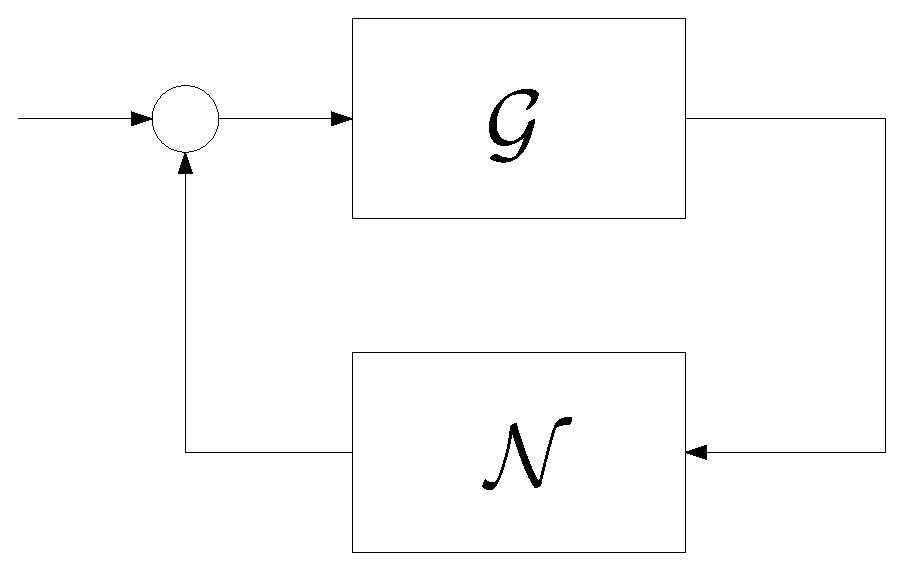
\includegraphics[width=0.75\columnwidth]{lure}
	\caption{A Lur'e system\label{fig:lur'e}}
\end{figure}
Models of this kind are known in the literature as Lur'e systems \cite{LurPos44} and a large number of real systems have this structure. Recent examples are provided by Atomic Force Microscopes \cite{SebSal01},\cite{SebGan05} and other Microelectromechanical systems \cite{WieSeb05}, \cite{SebWie08}, \cite{AgaSah08}.
Many studies targeted the problem of ``absolute stability'', where the global asymptotic stability of the origin is sought with respect to a class of nonlinear operators, and thus providing a robust notion of stability.
Classical results include the Popov (see \cite{Pop62}) and the circle criteria (see \cite{San64} and \cite{Zam66b}) that provide sufficient conditions for global asymptotic stability  when the nonlinearity is restricted to be  time-invariant and time varying respectively.
% For a recent survey of absolute stability results see \cite{Lib06}.
A relatively new approach involving only input-output maps is given by the Integral Quadratic Constraint (IQC) methods pioneered in \cite{MegRan97}. In this approach, a quadratic constraint is used to characterize the nonlinearity playing the role of the sector condition used in the other classical absolute stability criteria.
Since the sector relations can be derived as special IQC conditions, such an approach provides  a powerful unifying theoretical framework. Furthermore, it provides the powerful capability of seamlessly integrating different characterizations of the nonlinearity, as well.
When an equilibrium is not globally asymptotically stable, it is important for many practical issues to estimate its domain of attraction. Indeed, the domain of attraction represents the region of perturbations on the equilibrium which the system can absorb. Estimating a domain of attraction is a difficult problem to solve even from a numerical point of view, especially when the phase space has a large dimension.
Any approach based on simulation techniques would require a large number of systematic simulations with different initial conditions. An analytical, but more conservative method to estimate the domain of attraction is provided by the LaSalle theorem \cite{Khalil,Vidyasagar} which relies on the knowledge of a Lyapunov function.
Since both the circle and the Popov criteria rely on the construction of a Lyapunov function in order to prove global asymptotic stability, the same criteria can be suitably modified in order to obtain local results assuming that the nonlinearity satisfies local properties only \cite{Khalil}. Consequentely, an estimate of the attraction domain can be accomplished exploiting the Lyapunov function provided by these criteria in combination with the LaSalle theorem.
In order to reduce the conservativeness of this approach, in \cite{HuxHua04} an optimization technique based on LMI's is proposed. It is based on the computation of the largest contractively invariant ellipsoid of a fixed shape containing the equilibrium. We remind that an ellipsoid is contractively invariant if the derivative of its related quadratic form is negative along the system trajectories. The authors also prove that the convex hull of contractively invariant ellipsoids is an invariant contractive set contained in the domain of attraction.\\
In this paper, we propose a technique to improve the estimate of attraction domains. LMI's are a powerful tool to obtain a quadratic Lyapunov function which proves local stability of an equilibrium. However, in some situations, contractively invariant ellipsoids and their convex hull provide a conservative estimate of the attraction domain. This is due to the strong requirement of ``contractive invariance'': the ellipsoid must be an invariant set and also the derivative of the Lyapunov function along the contained trajectories must be strictly negative.
Conversely, we assume that an estimate of the attraction domain is already known. In order to show that a set is part of the attraction domain, it is sufficient to prove that all the trajectories starting from it reach the current estimate in a finite time.
This concept provides a method to iteratively improve the attraction domain estimate without limiting the analysis to contractively invariant sets.
In the paper we formalize this intuitive idea developing adequate theoretical tools in order to handle positively invariant sets. After developing a general theory, we only resort to the use of quadratic Lyapunov functions because of the computational appeal given by LMI solvers. We also introduce the concept of Biased Local Quadratic Constraint as a technical instrument to describe a nonlinearity. It is a general formulation of many quadratic constraints which are used to express conditions in many stability criteria (Circle, Popov, Zames-Falb). A more general relaxation of the Integral Quadratic Constraints (IQC's) introduced by \cite{MegRan97} could have been pursued. However this is beyond the main objectives of this short article.
The paper is structured as follows: in Section \ref{sec:probdef} the problem is formulated; in Section \ref{sec:prelimanaries} some preliminary results are illustrated; Section \ref{sec:theory} contains the general theoretical results; Section \ref{sec:LMI'n'IQC} combines the theory with LMI's and BLQC's as practical tools to construct Lyapunov functions; finally Section \ref{sec:numerical examples} shows the utility and limits of our techniques through two numerical examples, providing also a comparison with other techniques in the literature.

\section{Definitions and Notation}
\begin{dfn}
	Given a space $X$ with a metric $d$, we extend the definition of the metric to include the concept of distance between a point $x\in X$ and a set $A\subset X$ in the following way
	\begin{align}
		d(x,A):=\inf\{d(x,y)| y\in A\}.
	\end{align}
\end{dfn}
\begin{dfn}
	Given a metric space $X$ with a metric $d$ and a set $A \subseteq X$, we define the neighborhood of $A$ with radius $\eps$ as
	\begin{align}
		\mathcal{I}(A,\eps):=\{x\in X| d(x,A)<\eps \}.
	\end{align}
\end{dfn}

Consider a dynamical system $\mathcal{S}$ described by an initial condition problem
\begin{align}\label{eq:dynsys}
	\begin{array}{l}
		\dot x = f(t,x)\\
		x(t_0)=x_0
	\end{array}
\end{align}
with $f:\Re\times\Re^n\rightarrow\Re^n$ ``regular enough'' in order to guarantee the uniqueness of solutions.
Let $x(t):=\phi(t,t_0,x_0)$ be the trajectory related to the initial condition $(t_0,x_0)$.
% 	Suppose that the state $x$ of the system assumes values in a normed space $D$ and that $\phi(t,t_0,x_0)$ is the trajectory related to the initial condition $(t_0,x_0)$.
%
\begin{dfn}
	We say that $A$ is an Positively Invariant (PI) set for $\mathcal{S}$ if and only if, for all $t>t_0$ and for all $x_0 \in A$
	\begin{equation}\nonumber
		\phi(t,t_0,x_0) \in A \qquad \text{for all}~t>T.
	\end{equation}
\end{dfn}
% \begin{dfn}
% 	 We say that $E$ is an Eventually Positively Invariant (EPI) set for $\mathcal{S}$ if and only if, for all $t_0$ and for all $x_0 \in E$, there exists $T\geq t_0$ such that
% 	\begin{equation}\nonumber
% 		\phi(t,t_0,x_0) \in E \qquad \text{for all}~t>T.
% 	\end{equation}
% \end{dfn}
\begin{dfn}
	We say that $A$ is an attracting set for $\mathcal{S}$ if, for any $\eps>0$, there exist a $\delta=\delta(\eps)$ and a $T=T(\eps)$ such that
	\begin{equation}
		x(t_0)\in \mathcal{I}(A,\delta) \text{ implies }
			x(t) \in \mathcal{I}(A,\eps) \text{ for all } t>T.
	\end{equation}
\end{dfn}
\begin{dfn}
	We say that $A$ is an attractor if it is an attracting set that does not contain any other proper attracting subset.
\end{dfn}
\begin{dfn}
	Given an attracting set $A$, we define its domain of attraction as
	\begin{align*}
		& \mathcal{D}(A):=\{x_0\in\Re^n|\\
			& \forall\eps>0 \exists T=T(\eps,x_0), t>T \text{ implies } \phi(t,t_0,x_0)\in \mathcal{I}(A,\eps) \}
	\end{align*}
\end{dfn}
\begin{dfn}
	Let $P$ be a strictly positive $n\times n$ matrix and let $H$ be a real nonnegative value. We define
	\begin{equation}\nonumber
		\ellips_P(H)\coloneqq 
			\left\{ 
				x\in \Real^n : x^T P x \leq H
			\right\}.
	\end{equation}
\end{dfn}
\begin{dfn}
	Given a scalar function $V:\Re^n\rightarrow\Re$ we define
	\begin{equation}\nonumber
		\Omega_V(H)\coloneqq 
			\left\{ 
				x\in \Real^n : V(x) \leq H
			\right\}.
	\end{equation}
\end{dfn}


\begin{dfn}
	Given a constant matrix $\Sigma\geq 0$, we define the quadratic form $\sigma: \Real^n \times \Real^n \rightarrow \Real$
		\begin{equation}\nonumber
			\sigma(y,u)=
					\left(\begin{array}{c}
						y\\
						u
					\end{array}\right)^*
					\Sigma
					\left(\begin{array}{c}
						y\\
						u
					\end{array}\right).
		\end{equation}
	We say that a nonlinearity $\Xi(\cdot)$ satisfies the Biased Local Quadratic Constraint (BLQC) defined by $\sigma$ with bias $M>0$, if and only if
	\begin{equation}\label{eq:defLQC}
		\sigma(y(t),\xi(t)) + M\geq 0 \qquad \text{for all}~t>0
	\end{equation}
	for any signals $y(t),\xi(t)\in L_{2e}$, where $\xi(t)=\Xi(y(t))$.
	We also use the notation $\Csi\in BLQC(\sigma,M)$ and say that the matrix $\Sigma$ is the multiplier of the BLQC.
% 	If the BLQC is satisfied for all $M>0$, we say that (\ref{eq:defLQC}) is an Unbiased Local Quadratic Constraint (ULQC).
\end{dfn}


\section{Problem definition}\label{sec:probdef}
Let us consider a Lur'e system as depicted in Figure~\ref{fig:lur'e}.
% \begin{figure}[!h]
% 	\centering
% 	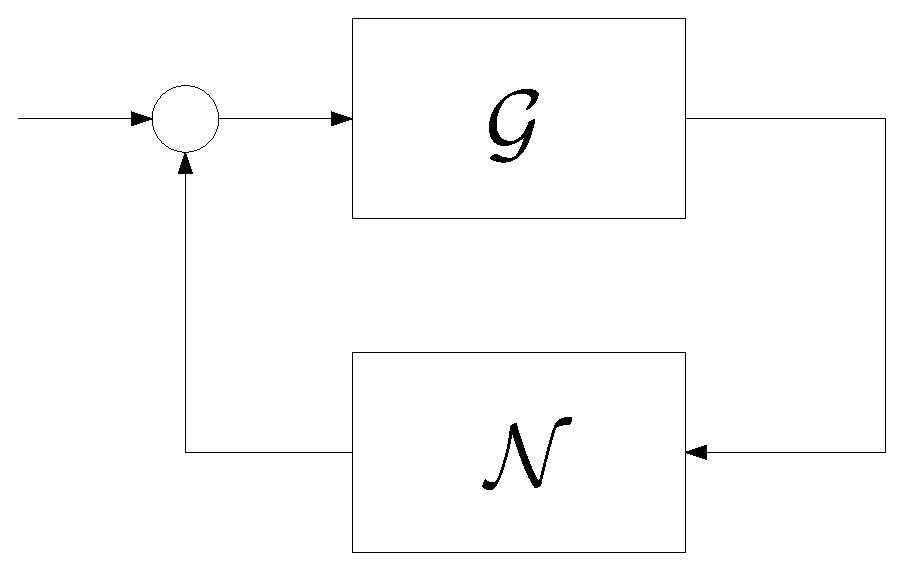
\includegraphics[width=0.75\columnwidth]{lure}
% 	\caption{A Lur'e System\label{fig:lur'e}}
% \end{figure}
Assume that the linear system $\mathcal{G}$ is proper with transfer function $G(s)$ and that the nonlinear block $\mathcal{N}$ can be described by a possibly time-varying operator $\Csi$. 
The differential equation representing such a feedback interconnection is symbolically expressed by
\begin{equation}\label{eq:symlur'e}
	y = G(d/dt)~\Csi(t, y(\cdot))
\end{equation}
where $y$ is the output of the system. Assume that the origin is a stable equilibrium for the system. The problem we are considering is to find an estimate of its attraction domain.

\section{Preliminary results}\label{sec:prelimanaries}
This section introduces some technical results needed to derive the main contributions of the paper.
% \begin{lem}\label{lem:ContainedQuadraticForms}
% 	Given two ellipsoids $\ellips_{P_A}(H_A)$ and
% 	$\ellips_{P_B}(H_B)$, we have that
% 	\begin{equation}
% 		\ellips_{P_A}(H_A) \supseteq \ellips_{P_B}(H_B)
% 		\Leftrightarrow \frac{H_A}{H_B}
% 			\geq \max \mathrm{eig}~P_B^{-1} P_A
% 	\end{equation}
% 	Moreover, if the inequality is strict, there is $\eps>0$ such that
% 	\begin{equation}
% 		\ellips_{P_A}(H_A) \supset \mathcal{I}(\ellips_{P_B}(H_B),\eps)
% 	\end{equation}
% \end{lem}
% \begin{proof}
% 	Without loss of generality we can assume $P_A$ and $P_B$
% 	symmmetric.
% 	From the spectral theorem, it is possible 
% 	to decompose $P_B$ in the form
% 	\begin{equation}
% 		P_B= S^2
% 	\end{equation}
% 	where $S$ is a symmetric and positive matrix.
% 	Define $y:=S x $, then
% 	\begin{align}
% 		\max_{x^T P_B x=1} x^T P_A x =
% 			\max_{y^T y=1} y^T S^{-T} P_A S^{-1} y
% 	\end{align}
% 	Consider the spectral decomposition of $S^{-T} P_A S^{-1}$
% 	\begin{equation}
% 		S^{-T} P_A S^{-1} = \Gamma \Theta \Gamma^T
% 	\end{equation}
% 	where $\Theta$ is diagonal and $\Gamma$ is ortonormal,
% 	then define $z:=\Gamma^T y $.
% 	We have
% 	\begin{equation}
% 		\max_{y^T y=1} y^T S^{-T} P_A S^{-1} y=
% 			\max_{z^T z =1} z^T \Theta z = 
% 				\max \mathrm{eig}~\Theta
% 	\end{equation}
% 	Since it is immediate to note that
% 	\begin{align}
% 		\mathrm{eig}~\Theta = 
% 			\mathrm{eig}~S^{-T} P_A S^{-1}=
% 			\mathrm{eig}~S^{-2} P_A =
% 			\mathrm{eig}~P_B^{-1} P_A
% 	\end{align}
% 	the proof is complete.
% \end{proof}
% The geometrical interpretation of Lemma 
% \ref{lem:ContainedQuadraticForms}
% is depicted in Figure \ref{fig:ContainedEllipses}.
% \begin{figure}[!h]
% % 	\psfrag{Pa}{$\ellips_A$}
% % 	\psfrag{Pb}{$\ellips_B$}
% % 	\psfrag{x1}{$x_1$}
% % 	\psfrag{x2}{$x_2$}
% 	\begin{center}
% 		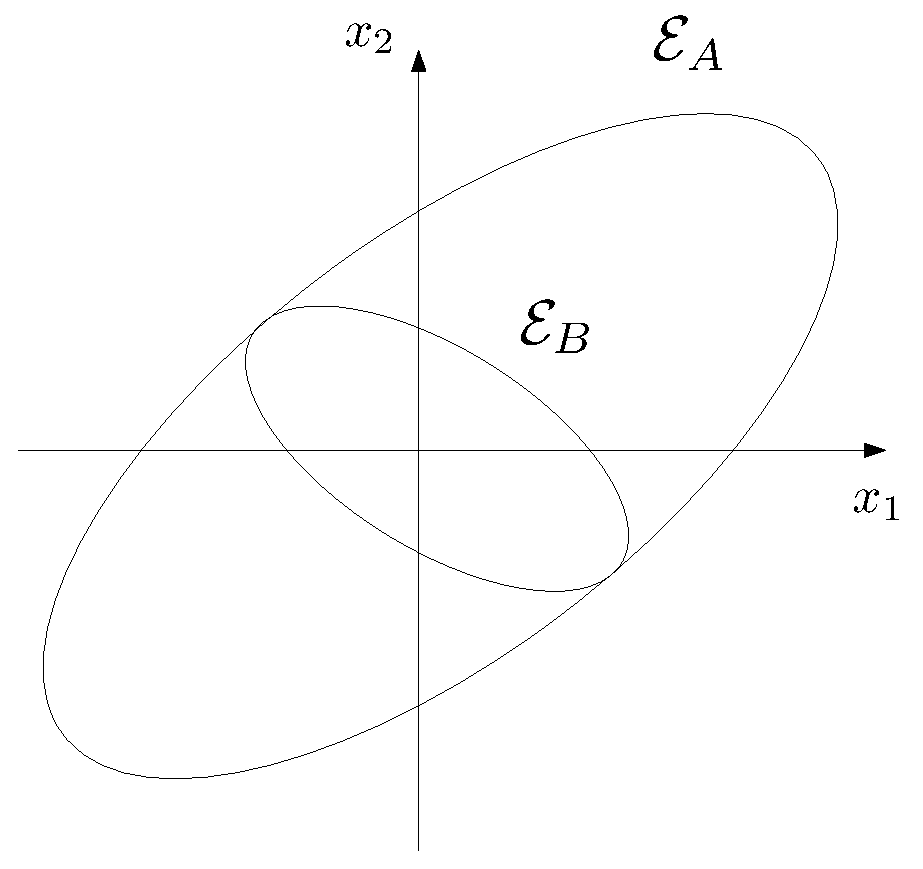
\includegraphics[width=0.75\columnwidth]{ContainedEllipses2}
% 	\end{center}
% 	\caption{\label{fig:ContainedEllipses}}
% \end{figure}
The following lemma provides a bound for the scalar output $y=Cx$ of a dynamical system when the state $x$ belongs to the ellipsoid $\ellips_P(H)$.
\begin{lem}\label{lem:BoundY}
Let us consider a positive symmetric matrix $P$, then it holds that
	\begin{align}
		\max_{x\in\mathcal{E}_P(H)} |Cx| 
			= \sqrt{H C P^{-1} C^T}
	\end{align}
\end{lem}
\begin{proof}
	The lemma is a trivial result of projective geometry.
\end{proof}
The following lemma is a technical result which will be exploited in the following section.
\begin{lem}\label{lem:equivalence Lyap and Norm}
	Assume that $V:\Re^n\rightarrow \Re$ is a continuous function and that $\Omega_V(H)$ is a compact set for any $H$. Then, for any $\eps>0$ there exists $H_{\eps}>H$ such that $x\in \Omega_V(H_{\eps})$ implies that
	\begin{align}
		d(x,\Omega_V(H_{\eps}))<\eps
	\end{align}
\end{lem}
\begin{proof}
	By contradiction there exists $\eps>0$ such that for any $H_{\eps}>H$ it is possible to find a $x\in \Omega_V(H_{\eps})$ with $d(x,\Omega_V(H_{\eps}))\geq\eps$.
	Consider the sequence $H_{n}=H+1/n$ and the related sequence $x_n$ such that
	\begin{align}
		d(x,\Omega_V(H))\geq\eps
	\end{align} 
	Since $\Omega_V(H+1)$ is a compact set, there exists a subsequence $x_{k_n}$  converging to $\hat x \in \Omega_V(H+1)$. By the continuity of $V$ we have that
	\begin{align}
		V(\hat x)= \lim_{n\rightarrow+\infty} V(x_{k_n})\leq
			\lim_{n\rightarrow+\infty} \left( H+\frac{1}{k_n}\right)=H
	\end{align}
	implying that $\hat x \in \Omega_V(H)$
	On the other hand we have
	\begin{align}
		0=d(\hat x, \hat x) =
			\lim_{n\rightarrow+\infty} d(x_{k_n},\hat x)\geq
			\liminf_{n\rightarrow+\infty} d(x_{k_n},\Omega_V(H))\geq
				\eps >0
	\end{align}
	which is a contradiction.
\end{proof}

% \begin{lem}\label{lem:matrioska}
% 	Consider a dynamical system as in (\ref{eq:dynsys}). Assume that $A_1$ and $A_2$ are two attractors. Assume also that $D_1$ and $D_2$ are contained in $\mathcal{D}(A_1)$ and $\mathcal{D}(A_2)$ respectively.
% 	If, for some $\eps>0$, $D_1 \supset \mathcal{I}(A_2,\eps)$ then $D_1 \cup D_2$ is contained in $\mathcal{D}(A_1)$.
% \end{lem}
% \begin{proof}
% 	We already know that $D_1$ is in $\mathcal{D}(A_1)$. Consider $x_0\in D_2$.
% 	Since $D_1 \supset \mathcal{I}(A_2,\eps)$, there will be a time $t$ such that $x(t):=\phi(t,t_0,x_0)\in D_1$.
% 	Since $D_1$ is in the attraction domain of $A_1$, we have that necessarily the trajectory $x(t)$ is attracted by it.
% \end{proof}
% \begin{lem}\label{lem:lyapliminf}
% 	Let $V(t)$ be a non-negative, continuous and differentiable function of time,
% 	defined for $t\geq 0$.
% 	Assume that there exists $r>0$ and $\sigma(t)$ such that
% 	\begin{equation}\label{eq:diffV_lem_liminf}
% 		\frac{dV}{dt}(t)<-r V(t)-\sigma(t),
% 	\end{equation}
% 	for all $V(t)\neq 0$.
% 	Assume also that $V(0)>0$ and there exists $M>0$ such that
% 	\begin{equation}
% 		\liminf_{t\rightarrow +\infty} \int_0^{t}[\sigma(\tau)+M]d\tau\geq 0.
% 	\end{equation}
% 	Then 
% 	\begin{equation}
% 		\liminf_{t\rightarrow +\infty} V(t)\leq \frac{M}{r}.
% 	\end{equation}
% \end{lem}
% \begin{proof}
% 	Given $\eps>0$, suppose there exists $t_2$ such that $t>t_2$ implies that $V(t)\geq \frac{M}{r}+\eps$.
% 	Since $\sigma(t)+M$ has non-negative liminf integral,
% 	there exists $t_1$ such that for $t>t_1$
% 	\begin{equation}
% 		\int_0^{~t}[\sigma(\tau)+M]d\tau\geq -\eps.
% 	\end{equation}
% 	Integrating both sides of (\ref{eq:diffV_lem_liminf}) with $t>\max(t_1,t_2)$
% 	\begin{equation}
% 		0\leq V(t)< V(0)-r\int_{0}^{t}V(\tau)d\tau+Mt+\eps<V(0)-r\eps~t+\eps.
% 	\end{equation}
% 	Choosing $t>(V(0)+\eps)/(r\eps)$ we have a contradiction.
% \end{proof}
% \begin{lem}\label{lem:conv_sigma^(-)}
% 	Let $\gamma(t)$ be piecewise continuous and assume that
% 	the Lebesgue integral of $\gamma$ exists on $[0,+\infty)$. Also assume that
% 	\begin{equation}\label{eq:liminfpositive}
% 		\liminf_{t\rightarrow +\infty}\int_0^t \gamma(\tau) d\tau=\alpha>0
% 	\end{equation}
% 	exists.
% 	Then
% 	\begin{equation}
% 		\lim_{t\rightarrow\infty}\int_0^{t}\gamma^{(-)}(\tau)d\tau<+\infty.
% 	\end{equation}
% \end{lem}
% \begin{proof}
% 	Since the Lebesgue integral exists, at least one of the two integrals
% 	\begin{equation}
% 		\int_0^{+\infty}\gamma^{(-)}(\tau)d\tau,
% 			\qquad
% 		\int_0^{+\infty}\gamma^{(+)}(\tau)d\tau
% 	\end{equation}
% 	is finite. Also the integrals
% 	\begin{equation}
% 		\int_0^{t}\gamma^{(-)}(\tau)d\tau,
% 			\qquad
% 		\int_0^{t}\gamma^{(+)}(\tau)d\tau
% 	\end{equation}
% 	are finite for all $t\geq 0$.
% 	By (\ref{eq:liminfpositive}), given $\eps>0$,
% 	there exists $T_{\eps}$ such that $t>T_{\eps}$ implies
% 	\begin{equation}
% % 		\inf_{t>T} 
% 			\int_0^{t}\gamma(\tau)d\tau>\alpha-\eps.
% 	\end{equation}
% 	With $\eps=\alpha/2$, we have that
% % 	\begin{equation}
% % 		\inf_{t>T} \int_0^{t}\gamma(\tau)d\tau>\frac{\alpha}{2}>0
% % 	\end{equation}
% % 	Thus
% 	\begin{equation}
% 		\int_0^{t}\gamma^{(+)}(\tau)d\tau>
% 			\int_0^{t}\gamma^{(-)}(\tau)d\tau+\frac{\alpha}{2}
% 	\end{equation}
% 	If
% 	\begin{equation}
% 		\lim_{t\rightarrow +\infty}\int_0^{t}\gamma^{(-)}(\tau)d\tau=+\infty
% 	\end{equation}
% 	we clearly have a contradiction of the hypothesis.
% \end{proof}
% 
% \begin{lem}\label{lem:Vlimsupbounded}
% 	Let $V(t)$ be a non-negative, continuous and differentiable function of time,
% 	defined for $t\geq 0$.
% 	Assume that there exists $r>0$ and $\sigma(t)$ such that
% 	\begin{equation}\label{eq:diffV_lem_lim}
% 		\frac{dV}{dt}(t)<-r V(t)-\sigma(t)
% 	\end{equation}
% 	for all $V(t)\neq 0$
% 	Assume also that $V(0)>0$ and
% 	\begin{equation}
% 		\liminf_{t\rightarrow +\infty} \int_0^{t}[\sigma(\tau)+M]d\tau> 0
% 	\end{equation}
% 	Then 
% 	\begin{equation}
% 		\limsup_{t\rightarrow +\infty} V(t)\leq \frac{M}{r}.
% 	\end{equation}	
% \end{lem}
% \begin{proof}
% % 	From (\ref{eq:diffV_lem_lim}) we have that the integral of $\sigma(t)$
% % 	can not diverge.
% 	Fix $\eps>0$ and define
% 	\begin{equation}
% 		\gamma(t):=\sigma(t)+M.
% 	\end{equation}
% 	By Lemma \ref{lem:conv_sigma^(-)}, we have that
% 	\begin{equation}
% 		\lim_{t\rightarrow +\infty}
% 			\int_0^{t}\gamma^{(-)}(\tau)d\tau<+\infty.
% 	\end{equation}
% 	Thus, by the theorem of Cauchy sequence, it is always possible to find $T_1$
% 	such that $T_1<t_a\leq t_b$ implies
% 	\begin{equation}
% 		\int_{t_a}^{t_b}\gamma^{(-)}(\tau)d\tau>-\eps/2.
% 	\end{equation}
% 	It follows from Lemma \ref{lem:lyapliminf}, that there exists a $t_0>T_1$ such that $V(t_0)<\frac{M}{r}+\eps$. We now want to prove that $t>t_0$ implies $V(t)<\frac{M}{r}+\eps$. By contradiction suppose there exists $t_2$ such that $t_2>t_0$ and $V(t_2)\geq\frac{M}{r}+\eps$.
% 	Because of the continuity of $V(x(\cdot))$ there must exist
% 	$t_1$ such that $t_0<t_1<t_2$, $V(t_1)=\frac{M}{r}+\eps/2$
% 	and $V(t)\geq \frac{M}{r}+\eps/2$ for $t_1\leq t \leq t_2$.
% 	Integrating (\ref{eq:diffV_lem_lim}) from $t_1$ to $t_2$
% 	\begin{align*}
% 		V(t_2)	&<V(t_1)-r\int_{t_1}^{t_2}V(t)d\tau
% 				+M(t_2-t_1) -\int_{t_1}^{t_2}\gamma(\tau)d\tau <\\
% 			&<\frac{M}{r}+\frac{\eps}{2}
% 				-r\int_{t_1}^{t_2}\left[V(t)-\frac{M}{r}\right]d\tau
% 				-\int_{t_1}^{t_2}\gamma^{(+)}(\tau)d\tau +\\
% 				&\qquad+\int_{t_1}^{t_2}\gamma^{(-)}(\tau)d\tau  \leq\\
% 			&\leq\frac{M}{r}+\frac{\eps}{2}+\frac{\eps}{2}=\frac{M}{r}+\eps
% 	\end{align*}
% 	which leads to a contradiction. This proves the lemma.
% \end{proof}

\section{Main Theoretical Results}\label{sec:theory}
The following theorem employs a scalar function $V$, defined on the state space, in order to detect positively invariant and attracting sets giving an estimate of their domain of attraction.
\begin{thm}\label{lem:contracting shell}
	Consider a dynamical system as in (\ref{eq:dynsys}) and a scalar function
	$V:\Re^n\rightarrow \Re, V\in C^{1}(\Re)$.
	Assume that
	\begin{align}
		x(t)\in\Omega_V(\overline H)\backslash \Omega_V(\underline H)
		\text{ implies } \dot V(x(t))<0
	\end{align}
	for some $\overline H > \underline H$ and that	$\Omega_V(H)$ is compact
% 	(boundedness is enough for FD spaces)
	for every $\underline H < H < \overline H$.
	Then
	\begin{itemize}
		\item $\Omega_V(H)$ is positively invariant
		\item $\Omega_V(\underline H)$ is an attracting set
		\item $\Omega_V(H)\subseteq \mathcal{D}(\Omega_V(\underline H))$.
	\end{itemize}
\end{thm}
\begin{proof}
	First, let us prove that $\Omega_V(H)$ is positively invariant.
	Fix $\eps>0$ and consider $x_0\in \Omega_V(H)$.
	By contradiction, there exists $t_3$ such that 
	$H<V(x(t_3)):=H^*<\overline H$.
	Consider
	\begin{align}
		& t_1:=\sup\{t|0<t<t_3, V(x(t))\leq H \}\\
		& t_2:=\inf\{t|t_1<t<t_3, V(x(t))\geq H^* \}\neq t_1.
	\end{align}
	Since $V(x(t))$ is a continuous function the sets are not empty and the definitions make sense. Note also that $t_1 < t < t_2$ implies
	$H<V(x(t))<H^*$.
	By the mean value theorem, we have that
	\begin{align}
		0<V(x(t_2))-V(x(t_1))=\int_{t_1}^{t_2}\dot V(x(t)) dt= \dot V(x(\hat t))(t_2-t_1)
	\end{align}
	for some $t_1< \hat t < t_2$, but this is a contradiction since $\dot V(x(\hat t))<0$.\\
	Now, let us prove that any trajectory with $x_0\in\Omega_V(H)$ is attracted to $\Omega_V(\underline H)$.
	Given $\eps>0$, it is always possible to find $H_{\eps}>\underline H$ such that
	\begin{align}
		x\in\Omega_V(H_\eps)\Rightarrow  d(x,\Omega_V(\underline H))<\eps.
	\end{align}
	Given $x_0\in\Omega_V(H)$, there exists $t>0$ such that $x(t)\in\Omega_V(H_\eps)$. Assume again by contradiction that it does not exist. This means that $V(x(t))> H_{\eps}$ for all $t$. Then we have
	\begin{align}
		dV/dt \leq -r := \min\{\dot V(x(t))| H_{\eps}\leq V(x(t)) \leq H\}<0.
	\end{align}
	Integrating both sides, we find a contradiction, since $V(x(t))$ should diverge to $-\infty$. Therefore there exists $t>0$ such that $x(t)\in\Omega_V(H_\eps)$. The fact that $\ellips_P(\underline H)$ is an attracting set follows from the positively invariance of $\ellips_P(H_{\eps})$.
\end{proof}
The most important property required from $V$ is to have a negative time derivative on the set $\Omega_V(\overline H)\backslash \Omega_V(\underline H)$ which can be interpreted as a ``shell'' in the phase space. Then, Theorem \ref{lem:contracting shell} intuitively states that such a shell is ``contractive'' in the sense that all trajectories in it approach its inner surface $\{x: V(x)=\underline{H}\}$.
A graphical representation of this intuition is given in Figure \ref{fig:contained lyap}.
\begin{figure}
	\centering
	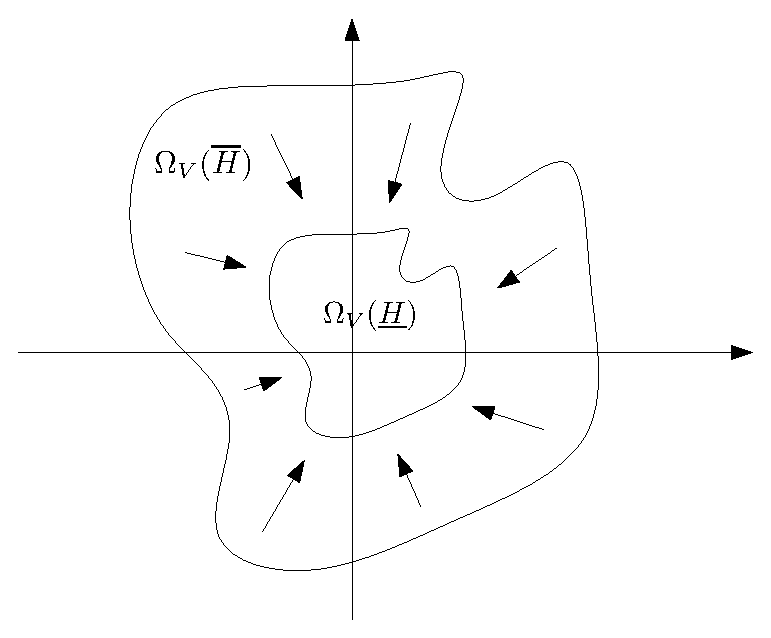
\includegraphics[width=0.9\columnwidth]{ContainedLyap}
	\caption{An intuitive representation of a ``contractive shell'' in the phase space
	\label{fig:contained lyap}}
\end{figure}
Note that Theorem \ref{lem:contracting shell} also provides a generalization of the 
classical Lyapunov theorem for asymtpotical stability when $\underline{H}=0$, $V(x)>0$ for any $x\neq 0$.

The following theorem provides a method to include level sets described by a scalar function $V_2$ into the attraction domain of attracting sets described by a different scalar function $V_1$.
\begin{thm}\label{thm:nestedLyap}
	Consider a dynamical system as in (\ref{eq:dynsys}) and two scalar functions
	$V_1, V_2:\Re^n\rightarrow \Re, V_i\in C^{1}(\Re)$.
	Assume that
	\begin{itemize}
		\item $x(t)\in\Omega_{V_2}(\overline H_2)\backslash \Omega_{V_2}(\underline H_2) \text{ implies } \dot V_2(x(t))<0$
		\item $x(t)\in\Omega_{V_2}(\underline H_2)\backslash \Omega_{V_1}(\underline H_1) \text{ implies } \dot V_1(x(t))<0$
		\item $\Omega_{V_1}(\underline H_1)$ is an attracting set
	\end{itemize}
	for some $\overline H_2 > \underline H_2$, $\underline H_1$.
	Then
	\begin{align}
		\Omega_{V_2}(H_2)\subseteq \mathcal{D}(\Omega_{V_1}(\underline H_1)).
	\end{align}
\end{thm}
\begin{proof}
	Given $H_2$ and $\eps_2>0$, from Lemma \ref{lem:contracting shell} we know that any solution $x(t)$ with initial condition in $\Omega_{V_2}(H_2)$ reaches the positively invariant set $\Omega_{V_2}(\underline H_2+\eps_2)$ at a time $t_1$.
	By the continuity of $\dot V_1(x(t))$ and Lemma \ref{lem:equivalence Lyap and Norm} it is possible to choose $\eps_2$ small enough, such that $\dot V_1(x(t))<0$ for any $x(t) \in \Omega_{V_2}(\underline H_2+\eps_2)\backslash \Omega_{V_1}(\underline H_1)$. Now let us prove that $x(t)$ is attracted by $\Omega_{V_1}(\underline H_1)$.
	By contradiction, assume that $x(t)$ is not attracted by $\Omega_{V_1}(\underline H_1)$. Thus, there is a $\eps_1>0$ such that $d(x(t),\Omega_{V_1}(\underline H_1))\geq \eps_1$ for any $t$ implying that $V(x(t))>\underline H_1$ for any $t$.
	Since $\Omega_{V_2}(\underline H_2+\eps_2)$ is a positively invariant set we have that $\dot V(x(t))<0$ for any $t>t_1$.
	Consider the relation
	\begin{align}
		&V(x(t))-V(x(t_1))=\\
		&\quad=\int_{t_1}^{t} \dot V(x(t))dt=\dot V(x(\hat t)) (t-t_1)<\eta(t-t_1).
	\end{align}
	This is a contradiction because it implies that $V(x(t))$ diverges to $-\infty$.
\end{proof}
Theorem \ref{thm:nestedLyap} provides a method to enlarge the attraction domain estimate of the attracting set $\Omega_{V_1}(\underline H_1)$ using level sets of the different Lyapunov function $V_2$. This is possible, according to the theorem hypothesis, when the contractive shell $\Omega_{V_2}(\overline H_2)\backslash\Omega_{V_2}(\underline H_2)$ has its inner surface contained in a region where $\dot V_1$ is negative.
An intuitive graphical representation is provided in Figure~\ref{fig:nested lyap}.
\begin{figure}
	\centering
	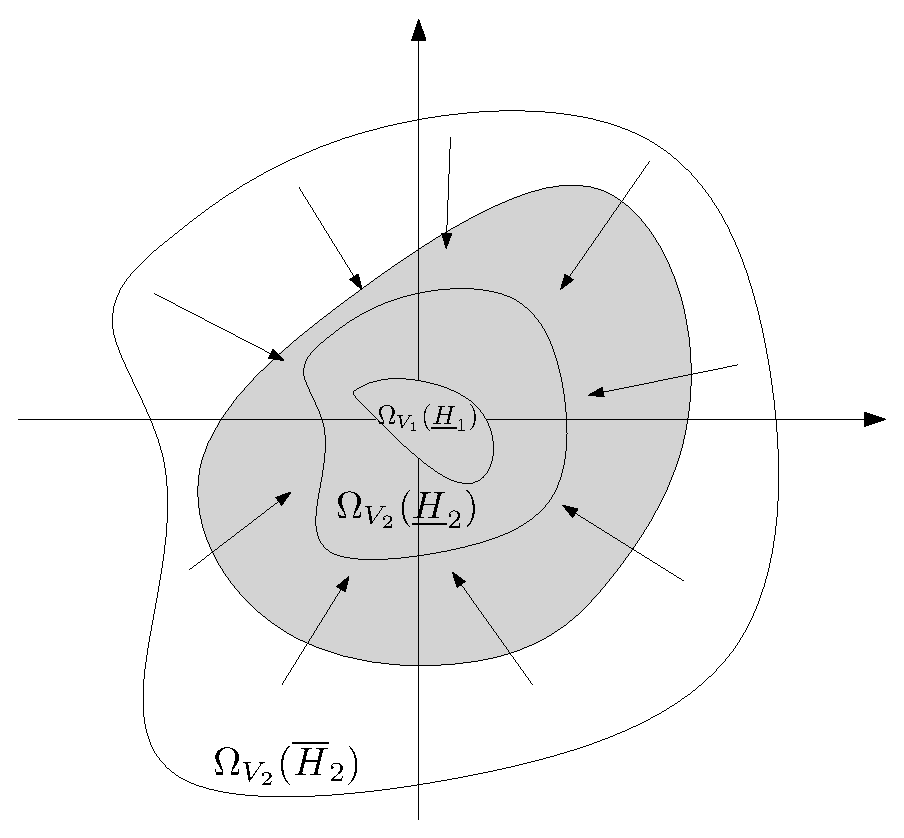
\includegraphics[width=0.9\columnwidth]{NestedLyap}
	\caption{An intuitive phase space representation of Theorem \ref{thm:nestedLyap}. The gray area represents the region where $\dot V_1$ is negative
	\label{fig:nested lyap}}
\end{figure}
It is important to stress that the set $\Omega_{V_2}(\overline H_2)$ is not required to be contractively invariant in order to be added to the estimate of attraction domain.

\section{LMI's and BLQC's to estimate domains of attraction}\label{sec:LMI'n'IQC}
In this section we exploit BLQC's and LMI's as practical tools to find attracting sets and estimate their domains.
We show the following results.
\begin{thm}\label{thm:contracting ellipsoidal shell}
	Let $\mathcal{S}$ be the Lur'e system described by~(\ref{eq:symlur'e}). Let $G(s)$ be a strictly proper transfer function and let $(A,B,C,0)$ be
	a minimal realization of $G(s)$ with state $x \in \Real^{n}$.
	Suppose that, for any $y$ such that $y^2<Y^2$, $\Csi$ satisfies the BLQC given by the quadratic form $\sigma$
	\begin{equation}
		\sigma(y,\xi)=
			\left(
				\begin{array}{c}
					y \\
					\xi
				\end{array}
			\right)^T
% 			\Sigma
			\left(
				\begin{array}{cc}
					Q	& S \\
					S^T	& R.
				\end{array}
			\right)
			\left(
				\begin{array}{c}
					y \\
					\xi
				\end{array}
			\right)
			\geq -M.
	\end{equation}
% 	with 
% 	\begin{equation}
% 		\Sigma=
% 		\left(
% 			\begin{array}{cc}
% 				Q	& S \\
% 				S^T	& R.
% 			\end{array}
% 		\right)
% 	\end{equation}
	Assume that there exists a solution $(P, r)$ to the following LMI
	\begin{equation}
		\left[
			\begin{array}{cc}
				A^TP+PA+C^TQC+rP	& PB+C^TS \\
				B^TP+S^TC		& R
			\end{array}
		\right] < 0
	\end{equation}
	with $P\in \Real^{n\times n}$, $P=P^T$, $P>0$, $r \in \Real^+$ and define
	\begin{align}
		& \underline{H} := \frac{M}{r}
		& \overline{H} := \frac{Y^2}{C P^{-1} C^T}.
	\end{align}
	If there exists $H$ such that $\underline H < H < \overline H$ , then  the set $\ellips_P(H)$ is a positively invariant set for $\mathcal{S}$. Moreover $\ellips_P(\underline H)$ is an attracting set and $\ellips_P(H)$ is contained in its attraction domain.
\end{thm}
\begin{proof}
	Define the Lyapunov function 
	\begin{equation}
		V(x)=x^TPx.
	\end{equation}
	The derivative of $V(x(t))$ along any trajectory satisfies
	\begin{align}
		dV/dt&=x^TA^TPx+x^TPAx+\xi^T B^T Px + x^T P B\xi=\\
			&=x^TA^TPx+x^TPAx+\xi^T B^T Px + x^T P B\xi+\\
			&\qquad +x^TC^TQCx+2x^TC^TS\xi+\xi^TR\xi-\sigma(y,\xi)\leq\\
			&\leq -r x^TPx -\sigma(y,\xi)
% 			\leq -r x^TPx +M.
	\end{align}
	Observe that the hypothesis of Theorem \ref{lem:contracting shell} are satisfied, so the assertion is proven.
\end{proof}
The following theorem is the main contribution of the paper providing an iterative technique to enlarge the estimate of a domain of attraction using $N$ different scalar functions.
\begin{thm}\label{thm:nested ellipsoidal Lyap}
	Let $\mathcal{S}$ be the Lur'e system described by~(\ref{eq:symlur'e}). Let $G(s)$ be a strictly proper transfer function and let $(A,B,C,0)$ be a minimal realization of $G(s)$ with state $x \in \Real^{n}$.
	Suppose that, for $i\in\{1,2,...,N\}$, $y(t)^2<Y_i^2$ implies  $\Xi\in BLQC(\sigma_i,M_i)$ where
	\begin{align}
		\sigma_i(y,\xi)=
			\left(
				\begin{array}{c}
					y \\
					\xi
				\end{array}
			\right)^T
% 			\Sigma
			\left(
				\begin{array}{cc}
					Q_i	& S_i \\
					S^T_i	& R_i.
				\end{array}
			\right)
			\left(
				\begin{array}{c}
					y \\
					\xi
				\end{array}
			\right)
			\geq -M_i
	\end{align}
	and $Y_i<Y_{i+1}$ for $i=\{i=1,...,N-1\}$.
	Assume that there exist solutions $(P_i, r_i)$ to the LMI's
	\begin{equation}
		\left[
			\begin{array}{cc}
				A^TP_i+P_iA+C^TQ_iC+rP_i	& P_iB+C^TS_i \\
				B^TP_i+S_i^TC			& R_i
			\end{array}
		\right] < 0
	\end{equation}
	with $P_i\in \Real^{n\times n}$, $P_i=P_i^T$, $P_i>0$, $r_i \in \Real^+$ and define
	\begin{align}
		& \underline{H_i} := \frac{M_i}{r_i}
		& \overline{H_i} := \frac{Y_i^2}{C P_i^{-1} C^T}.
	\end{align}
	Then, if $\underline{H}_{i+1} C P_{i+1}^{-1} C^T < Y_i^2$,
	\begin{align}
		\ellips_{P_N}(H_N)\subseteq \mathcal{D}(\ellips_{P_1}(\underline H_1)).
	\end{align}
	for any $H_N<\overline{H}_N$.
\end{thm}
\begin{proof}
	Consider the Lyapunov functions
	\begin{align}
		V_i(x)=x^T P_i x
	\end{align}
	and compute their derivatives along their trajectories
	\begin{align*}
		dV_i/dt&=x^TA^TP_ix+x^TP_iAx+\xi^T B^T P_i x + x^T P_i B\xi=\\
			&=x^TA^TP_i x+x^TP_i Ax+\xi^T B^T P_i x + x^T P_i B\xi+\\
			&\qquad +x^TC^TQ_i Cx+2x^TC^TS_i\xi+\xi^TR_i\xi-\sigma(y,\xi)\leq\\
			&\leq -r_i x^TP_i x -\sigma_i(y,\xi)
% 			\leq -r x^TP_i x +M_i.
	\end{align*}
	Observe that the hypothesis of Theorem \ref{thm:nestedLyap} are satisfied for any set of parameters with contiguous indexes $(i, i+1)$. Thus, the assertion is proven.
\end{proof}

\section{Numerical examples}\label{sec:numerical examples}

\subsection{Step by step application of Theorem \ref{thm:nestedLyap}}
This example has the objective to exemplify the basic ideas behind Theorem \ref{thm:nestedLyap} following a step by step procedure. We will use the Nyquist plot and the circle criterion as tools to help the intuitive reasoning.
Consider a physical system modeled by the transfer function
\begin{align}\label{eq:G(s) ex02}
	&\dot x =\left(\begin{array}{cc}
		0 & -50\\ 1 & 1
		\end{array}\right)+
		\left(\begin{array}{c}
		-10\\ 10 
		\end{array}\right)u\\
	& y = (0 \quad 1)x
\end{align}
% \begin{align}\label{eq:G(s) ex02}
% 	&G(s)=\frac{10(s-1)}{(s^2-s+50)}
% \end{align}
and assume a saturation on the actuators
\begin{align}
	u=\sat_L(v):=\min\{|v|,L\}\sgn(v)
\end{align}
with saturation level $L=5$ and a nonlinear static controller of the form
\begin{align}\label{eq:cubic controller}
	v=K_1 y+ K_3 y^3.
\end{align}
with $K_1=1.31$ and $K_3=3$.
A controller as (\ref{eq:cubic controller}) can be useful in situations where it is important to obtain local performances in the neighborhood of the equilibrium ($v\simeq K_1 y$) and at the same time it is desirable to have a prompter response when the system state is far from it. The linear transfer function $G(s)$ is not stable so it is not possible to globally stabilize if because of the input saturation. We want to obtain an estimate of the attraction domain using the criterion proposed in the previous section.
The Nyquist plot of (\ref{eq:G(s) ex02}) is depicted in Figure~\ref{fig:nyquist ex 02}.
\begin{figure}
	\centering
	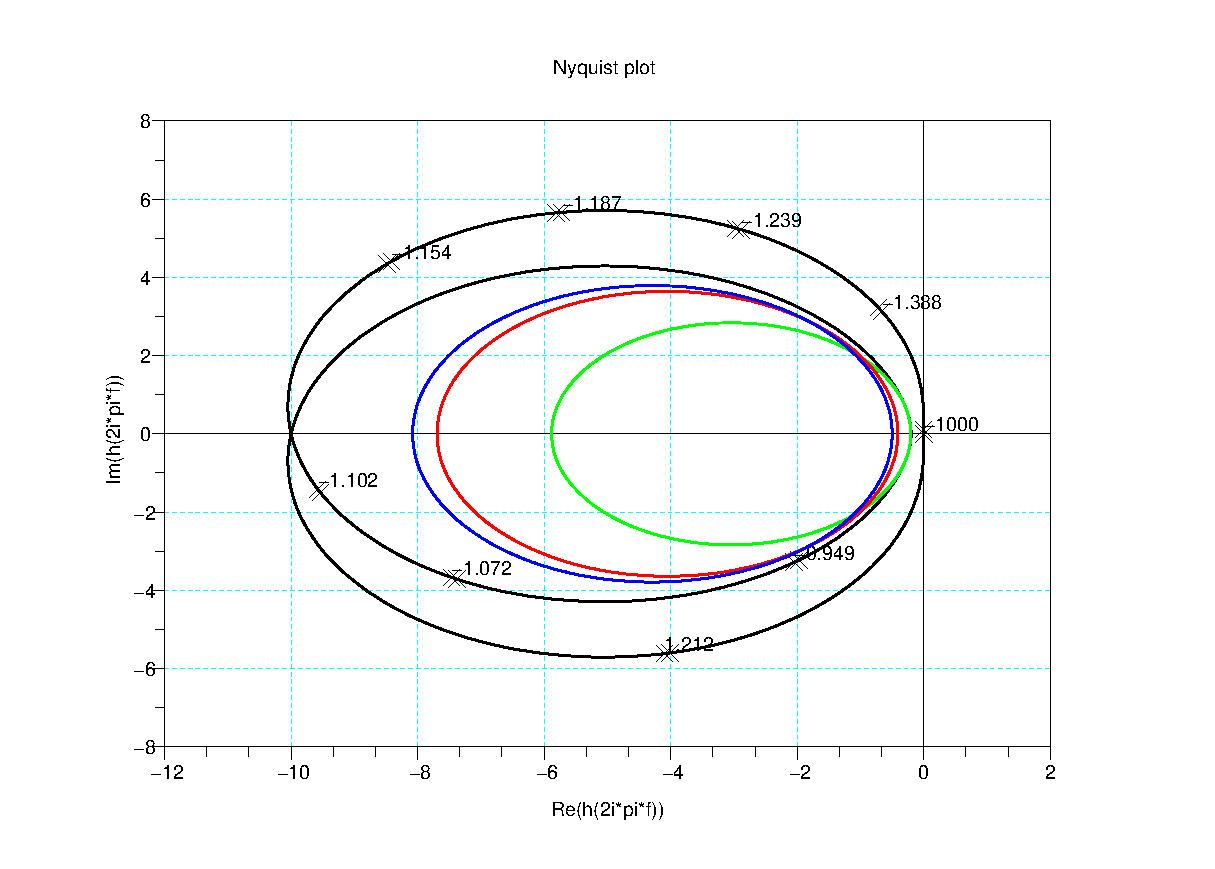
\includegraphics[width=0.9\columnwidth]{nyquist_ex02}
	\caption{The Nyquist plot of the linear transfer function (\ref{eq:G(s) ex02}) (black) and the circles associated to the sectors $S_1$ (green), $S_2$ (red) and $S_3$ (blue) as in example A.
	\label{fig:nyquist ex 02}}
\end{figure}
% The system is unstable and we want to design a feedback controller in order to stabilize it. At the same time, for practical purposes, a large domain of attraction is a desiderable feature.
% The choice of a linear gain $K_1$ is subjected to the constraint $K_1\in [0.1,5]$ in order to make the system stable. The extreme values of the Hurwitz sector make the system close to unstable conditions.
% Moreover, the saturation on the actuator poses limitations on the attraction domain of the system: when the state is far from the origin, the controller action is limited by the saturation contraint, thus the state diverges.
% Larger values of $K_1$ provide a prompter response, so they are expected to enlarge the attraction domain.
% Figure \ref{AD linear} shows the attraction domain for different values of $K_1$. As expected larger values of $K_1$ provide larger attraction domains.
% \begin{figure}
% 	\centering
% 	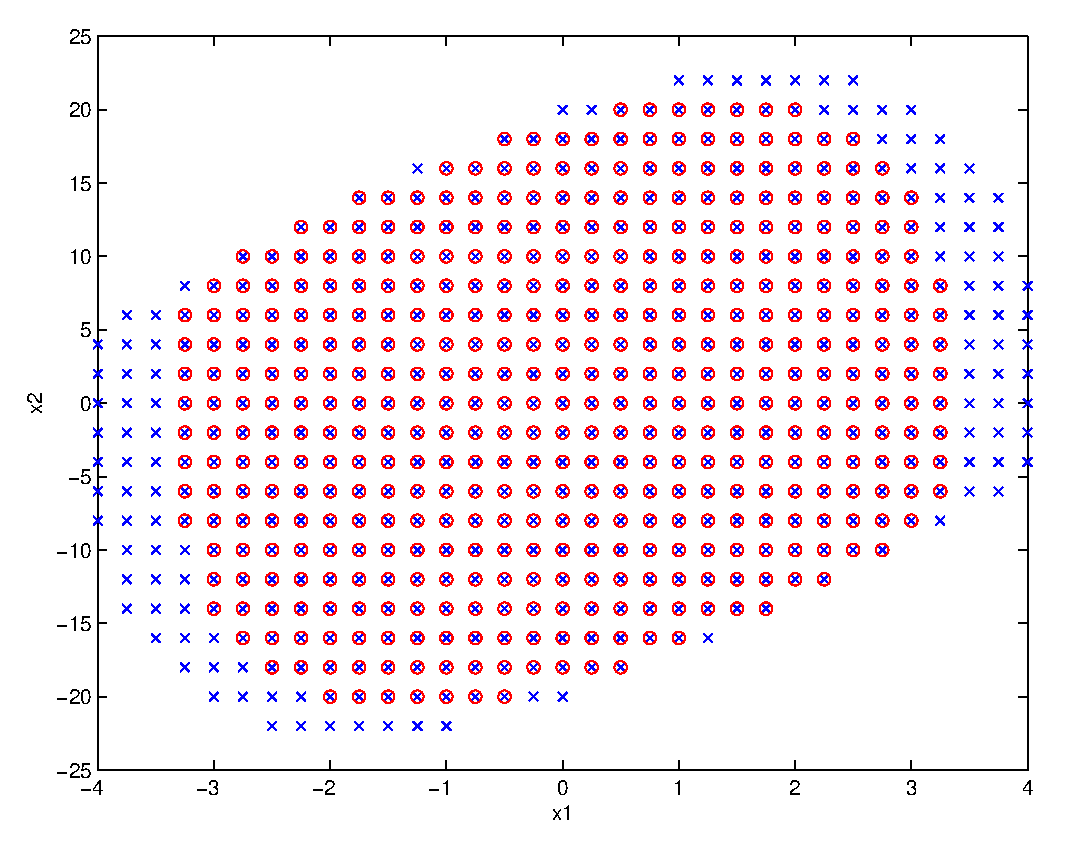
\includegraphics[width=0.9\columnwidth]{AD_linear}
% 	\caption{Attraction Domain for $K=0.5$ and $K=0.95$ \label{AD linear}}
% \end{figure}
% The choice of a linear static controller necessarily needs to face a trade-off between local convergence performances and the size of the attraction domain.\\
% Conversely, the choice of a nonlinear controller helps to mitigate the trade-off.
% We will design a nonlinear static controller of the form
% \begin{equation}
% 	n(y)=\sat_L(K_1 x + K_3 x^3).
% \end{equation}
% The parameter $K_1$ associated to the linear part of $n$ will take into account the local convergence performances while the parameter $K_3$ will be used to increase the estimate of the attraction domain according to our technique.
% Assume that $K_1=1.32$ satisfies the local performance specifications (TODO: try a pole placement).\\
We can use the circle criterion in order to find an estimate of the domain of attraction. As it is shown in Figure \ref{fig:nyquist ex 02} the sector $\mathcal{S}_1:=(\alpha_1,\beta_1)=(0.17, 4.85)$ is a stability sector for the system.
It can be verified that $0\leq K_3 \leq 3$ implies $n(y):=\sat_L(v(y))\in\mathcal{S}_1$
for $|y|<L/\alpha_1 = Y_1 \simeq 29.411$.
In the BLQC formulation the sector condition of the circle criterion is equivalent to $n(y)\in BLQC(\sigma_1,0)$ with multiplier
\begin{align}
	\Sigma_1=	\left(\begin{array}{cc}
				-\alpha_1\beta_1 & -(\alpha_1+\beta_1)\\ -(\alpha_1+\beta_1) & -1
			\end{array}\right).
\end{align}
A standard way to estimate the domain of attraction is given by the LaSalle theorem exploiting the quadratic Lyapunov function provided by the circle criterion
(see the green ellipsoid in Figure~\ref{fig:AttractionDomains}).
\begin{figure}
	\centering
	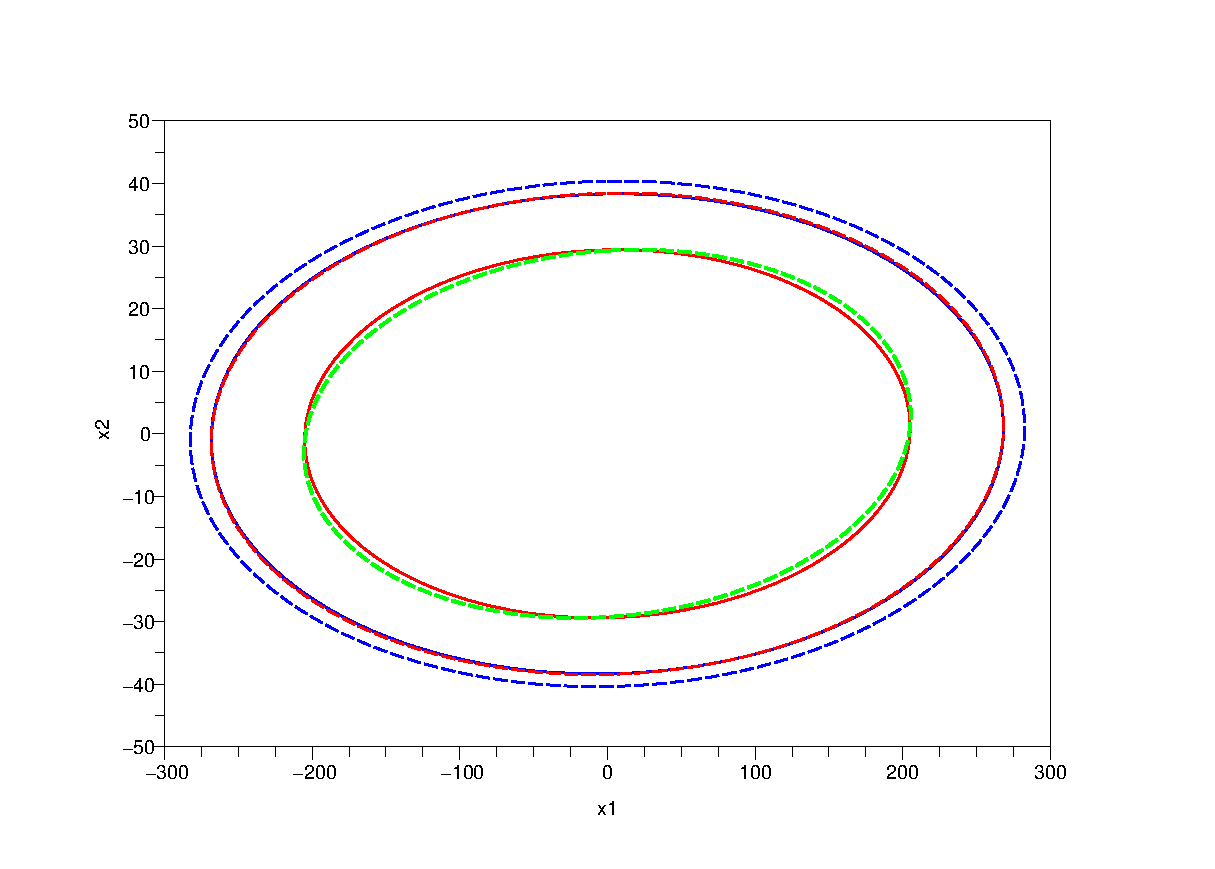
\includegraphics[width=0.9\columnwidth]{AttractionDomains}
	\caption{Attraction Domain Estimates\label{fig:AttractionDomains}.}
\end{figure}
It is possible to obtain a better estimate of the attraction domain. We note that $n(y)\in BLQC(\sigma_2,M_2)$ where the BLQC multiplier is
\begin{align}
	\Sigma_2=	\left(\begin{array}{cc}
				-\alpha_2\beta_2 & -(\alpha_2+\beta_2)\\ -(\alpha_2+\beta_2) & -1
			\end{array}\right).
\end{align}
for $\alpha_2=0.13$, $\beta=2.44$, $M_2=11.7$ and for any $|y|<L/\alpha_2=: \overline Y_2 \simeq 38.461$. Solving the associated LMI's we obtain a Lyapunov function $V_2=x^TP_2x$ which allows to conclude that eventually $|y(t)|<\underline Y_2 \simeq 29.39 < \overline Y_1$ if $x$ belongs to an ellipsoid $\ellips_{P_2}(\overline H_2)$.
Thus, $\ellips_{P_2}(\overline H_2)$ (the larger red ellipsoid in Figure~\ref{fig:AttractionDomains}) is in the attraction domain.
The same procedure can be repeated a third time noting that 
$n(y)\in BLQC(\sigma_3,M_3)$ for $\alpha_3=0.1238$, $\beta=2.00$, $M_2=13.992$
for $|y|<L/\alpha_3=: \overline Y_3 \simeq 40.38$. In an analogous way we find that $y(t)$ is eventually bounded by $\underline Y_3 \simeq 38.34$. Then the ellipsoid $\ellips_{P_3}(\overline H_3)$ (the larger blue ellipsoid in Figure~\ref{fig:AttractionDomains}) is in the attraction domain.

\subsection{Contractively invariance vs. combined Lyapunov functions}
In \cite{HuxHua04} a technique to estimate attraction domains is described. Such a technique estimates attraction domains using contractively invariant ellipsoids. The following example demonstrates that the adoption of contractively invariant ellipsoids can be a limiting choice in some situations.
Consider the following system (which admits a Lur'e representation)
\begin{align}
	&\dot x =\left(\begin{array}{cc}
		-\rho & 1\\ -1 & -\rho
		\end{array}\right)+
		\left(\begin{array}{c}
		-1\\ 0 
		\end{array}\right)u\\
	& y = (0 \quad 1)x\\
	& u = -n(y)=-\frac{y^2(y^2+2)}{(y^2+1)^2}y
\end{align}
with $\rho>0$.
Using the Lyapunov function (which is not quadratic)
\begin{align}
	V(x)=x_1^2+x_2^2+\frac{x_2^4}{x_2^2+1}
\end{align}
we can prove that the origin of the system is globally asymptotically stable for any positive $\rho$.
However, for $\rho<\overline \rho_{CI} \simeq 0.204$, it can be proved that there exists a positive value $X_2>0$ such that any contractively invariant ellipsoid must lie in the strip $|x_2|\leq X_2$. Thus, the approach in \cite{HuxHua04} can not establish global asymptotical stability. Conversely, we can show that the technique presented in this paper (for $N=2$) can prove that the domain of attraction is $\Re^2$ even for values of $\rho > \overline \rho_{I}\simeq 0.11$.
% with $\overline \rho_{I} < \overline \rho_{CI}$.

\subsubsection{Computational part}
~\\
Consider Theorem \ref{thm:nested ellipsoidal Lyap} with
\begin{equation}
	\begin{array}{llll}
	M_1=0,		&\alpha_1=1, 	&\beta_1=1.67,	& Y_1=1.4, \\
	M_2=0.09, 	&\alpha_2=1.6, 	&\beta_2=2,	& Y_2=+\infty,
	\end{array}
\end{equation}
% and with
\begin{equation}
	\Sigma_i=	\left(\begin{array}{cc}
				-\alpha_i\beta_i & -(\alpha_i+\beta_i)\\ -(\alpha_i+\beta_i) & -1
			\end{array}\right),
\end{equation}
and solve the associated LMI's. The solutions we found for $\rho=0.11$ using the Scilab Lmi solver are
\begin{align}
	P_1=	\left(\begin{array}{cc}
			0.2384 & 0.0022\\ 0.0022 & 0.5568
		\end{array}\right),
	&P_2=	\left(\begin{array}{cc}
			0.2187 & 0.0084\\ 0.0084 & 0.6131
		\end{array}\right).
\end{align}
Since the hypothesis are verified, the set $\ellips_{P_2}(H_2)$, for any $H_2<\overline{H}_2=+\infty$, is in the attraction domain of the attracting set $\ellips_{P_1}(0)=\{0\}$. This is equivalent to global asymptotic stability for the origin.

\section{Conclusions}
In this paper, we have developed a technique to reduce the conservativeness of attraction domain estimates in Lur'e systems. The novelty of our approach lies in the fact that the sets we are considering are invariant but not necessarily contractively invariant as in other criteria. A comparison of our method with other results in the literature is presented using numerical examples.

\section*{Acknowledgments}
The authors are grateful to the developers of Scilab at INRIA. The numerical implementations of the techniques described in this paper have been realized thanks to their valuable work.

\bibliography{abstab}
\end{document}